\section{Empirical Evaluation and Live Cyber-Range Benchmarks}
\label{sec:evaluation}

We separate certificate identity, temporal attribution and graph hardening. The primary questions are:
\begin{itemize}
\item \textbf{RQ1 (Attribution):} Which certificate-specific links and mutation overlaps are supported under incomplete identifiers, optional-source faults and time uncertainty?
\item \textbf{RQ2 (Collection and retention):} What costs are measured for replay, offline reasoning and periodic collection, and which costs remain unmeasured?
\item \textbf{RQ3 (Remediation):} What pair-disconnection values, cut counts and optimality gaps occur under assigned costs and immutable edges?
\end{itemize}
The optional GNN diagnostic is reported in Appendix~\ref{sec:graph_evaluation}. It is not evidence of certificate exploitation or a prerequisite for the live evaluation. Unless otherwise stated, dispersions are population standard deviations of the finite evaluated seeds, folds or graphs; paired tests use the saved per-graph observations.

\subsection{Experimental Setup}
\paragraph{Synthetic Identity Graphs} The class-balanced static benchmark uses 700 class-balanced synthetic identity graphs. Additional graph sizes are used in the separate scalability experiments. Neither the class proportions nor the graph generator constitute a measured enterprise distribution. The matched gating audit uses the existing two-step implementations with fixed source snapshots and separately recorded training, validation, and test inputs.

\paragraph{Controlled Windows testbeds} We use a virtualized Game of Active Directory (GOAD) cyber-range. Inventory of the restored DC and CA identifies Windows Server 2016 Standard Evaluation, build 14393. The two nodes are:
\begin{itemize}
    \item \texttt{DC03} (\texttt{essos.local}): Active Directory Domain Controller, Kerberos KDC, and LDAP directory.
    \item \texttt{SRV03} (\texttt{braavos.essos.local}): Certificate Authority running Microsoft Active Directory Certificate Services.
\end{itemize}
The split-actor case uses domain accounts \texttt{ESSOS\textbackslash khal.drogo} and \texttt{ESSOS\textbackslash viserys.targaryen}. Original disk images were read-only; execution used writable overlays. The capture pipeline runs non-interactively, while restoring the old VM images required console-assisted recovery. A second, independently provisioned forest uses Windows Server 2019 build 17763.4974, its own CA and ordinary enroller, and host-generated SHA-256-signed requests. This measured 2023 patch level is not described as a current patched configuration.

\subsection{RQ1 and RQ2: Provenance Evidence and Collection Cost}
\label{sec:streaming_evaluation}
We separate seven archived trace files, one new outcome-checked Windows case, a synthetic attribution confirmation study, and the earlier $10,182$-event trace-driven synthetic stress stream. Their outcome definitions and evidence levels differ; scenario filenames are not independent success labels.

\begin{table}[tbp]
\centering
\caption{Audit of Seven Archived GOAD Files: 586 Raw Events. Linkage concerns the captured certificate issuance-to-use chain. Attack recall is not established for any file.}
\label{tab:live_traces}
\evidencetable
\setlength{\tabcolsep}{2pt}
\begin{tabular}{@{}>{\raggedright\arraybackslash}p{.32\linewidth}r>{\raggedright\arraybackslash}p{.51\linewidth}@{}}
\toprule
Scenario & Events & Captured linkage \\
\midrule
Normal enrollment & 89 & No consistent captured issuance \\
ESC4 rollback & 90 & No consistent captured issuance \\
ESC6 CA flag scenario & 172 & KDC failure result \texttt{0x42} \\
ESC9 UPN swap & 94 & No consistent captured issuance \\
ASN.1 SAN concealment & 88 & No consistent captured issuance \\
Admin typo rollback & 6 & No certificate-use observation \\
Split-actor scenario & 47 & Resolved observed linkage \\
\bottomrule
\end{tabular}
\end{table}

\begin{table}[tbp]
\centering
\caption{Trace-Driven Synthetic Streaming Benchmark ($10,182$ Events, 48 Generated Attack Instances, 50 Simulated Maintenance Windows). The table measures the streaming implementation, not the constraint reference.}
\label{tab:cipg_stress}
\evidencetable
\setlength{\tabcolsep}{2pt}
\begin{tabular}{@{}>{\raggedright\arraybackslash}p{.30\linewidth}*{5}{>{\centering\arraybackslash}p{.12\linewidth}}@{}}
\toprule
Pipeline & \textbf{Prec.} & \textbf{Recall} & \textbf{F1} & \makecell{Maint.\\FPR} & \makecell{Event\\FPR} \\
\midrule
Snapshot rollback & 19.35\% & 25.00\% & 21.82\% & 100.0\% (50/50) & 0.49\% \\
CA event 4887 & 88.24\% & 58.33\% & 70.16\% & 0.00\% (0/50) & 0.00\% \\
\makecell[l]{CIPG, default\\$\Delta_{\text{poll}}=5$ s} & \textbf{92.16\%} & \textbf{97.92\%} & \textbf{94.95\%} & \textbf{8.00\% (4/50)} & \textbf{0.0395\%} \\
\makecell[l]{CIPG, fast\\$\Delta_{\text{poll}}=1$ s} & \textbf{92.31\%} & \textbf{100.00\%} & \textbf{96.00\%} & \textbf{8.00\% (4/50)} & \textbf{0.0395\%} \\
\bottomrule
\end{tabular}
\end{table}

\begin{table}[tbp]
\centering
\caption{2D Sensitivity Matrix: Precision above recall (\%) across Correlation Horizon ($\Delta t$) and CA Jet DB Polling Lag ($\Delta_{\text{poll}}$).}
\label{tab:sensitivity_matrix}
\evidencetable
\setlength{\tabcolsep}{2pt}
\begin{tabular}{@{}lcccc@{}}
\toprule
\makecell{Window (s)\\FPR (\%)} & \makecell{Poll\\1 s} & \makecell{Poll\\5 s} & \makecell{Poll\\15 s} & \makecell{Poll\\60 s} \\
\midrule
\makecell[l]{10\\0.0} & \makecell{100.0\%\\100.0\%} & \makecell{100.0\%\\97.92\%} & \makecell{100.0\%\\89.58\%} & \makecell{100.0\%\\89.58\%} \\
\makecell[l]{30\\6.0} & \makecell{94.12\%\\100.0\%} & \makecell{94.00\%\\97.92\%} & \makecell{93.48\%\\89.58\%} & \makecell{93.48\%\\89.58\%} \\
\makecell[l]{60\\8.0} & \makecell{92.31\%\\100.0\%} & \makecell{92.16\%\\97.92\%} & \makecell{91.49\%\\89.58\%} & \makecell{91.49\%\\89.58\%} \\
\makecell[l]{300\\8.0} & \makecell{92.31\%\\100.0\%} & \makecell{92.16\%\\97.92\%} & \makecell{91.49\%\\89.58\%} & \makecell{91.49\%\\89.58\%} \\
\makecell[l]{900\\8.0} & \makecell{92.31\%\\100.0\%} & \makecell{92.16\%\\97.92\%} & \makecell{91.49\%\\89.58\%} & \makecell{91.49\%\\89.58\%} \\
\bottomrule
\end{tabular}
\end{table}

\paragraph{Collection delay and attribution trade-offs}
As documented in Table~\ref{tab:cipg_stress} and Table~\ref{tab:sensitivity_matrix}, in the configured synthetic CA/KDC workload, operational performance is governed by two orthogonal systems dimensions:
\begin{itemize}
    \item \textbf{Correlation horizon and collisions:} The generator fixes 2,000 renewal arrivals uniformly over the simulated duration $T$; it does not sample an unconditional 2,000-per-hour Poisson process. Each renewal selects a maintenance template with probability $0.055$, uniformly among 15 templates; otherwise it selects the machine template. For one maintenance template and a horizon $\Delta\le T$, the simplified matching-arrival probability is $1-(1-0.055\Delta/(15T))^{2000}$, before any additional principal or detector conditions. Thus an aggregate arrival count cannot be substituted for the rate of matching template/principal events. In the seeded realization, the sensitivity query reports 0/50 collisions at 10~s, 3/50 at 30~s and 4/50 from 60~s onward. These are observed finite-workload counts, not estimates of collision-free production operation. Generated maintenance durations lie in $[10,35]$~s. The plateau concerns the retained workload and query; it is not a universal Poisson law.
    \item \textbf{CA Database Polling Lag ($\Delta_{\text{poll}}$) vs. False Negatives:} Because KDC Event 4768 omits SubjectKeyIdentifier (SKID), linking these selected issuance and authentication records requires the CA database or an equivalent captured certificate-identity bridge. When an attacker's PKINIT execution delay $\delta_{\text{pkinit}} \sim \text{LogNormal}(1.2, 0.8)$ executes before the next polling tick ($t_{\text{auth}} + \Delta_{\text{watermark}} < t_{\text{poll}}$), the join keys remain un-enriched at evaluation time, producing unresolved links at the fixed evaluation deadline. At $\Delta_{\text{poll}} = 1.0\text{s}$, CIPG achieves $100.00\%$ recall ($48/48$). At default $\Delta_{\text{poll}} = 5.0\text{s}$, CIPG achieves $97.92\%$ recall ($47/48$). At $\Delta_{\text{poll}} \in \{15\text{s}, 60\text{s}\}$, rapid attacks beat the polling cycle, resulting in $89.58\%$ recall ($43/48$).
\end{itemize}

\paragraph{Ingestion Throughput and Memory Profiling}
On the finite replay workload:
\begin{itemize}
    \item \textbf{Throughput:} The saved streaming benchmark reports \textbf{13,192.4 events/second} (771.81~ms) on the configured synthetic stream. This excludes a demonstrated end-to-end Windows collection/deployment pipeline and is not a throughput measurement of the constraint reference reasoners.
    \item \textbf{Memory Footprint:} The streaming result reports \textbf{6.91 MB}. A finite-run measurement does not establish bounded retained memory as the certificate history grows.
    \item \textbf{Meta-Node Compression:} Meta-node compacting collapsed 10,182 raw elements into 2,382 compressed elements, achieving a \textbf{76.61\% reduction in graph size} in the benchmark's repeated-event representation.
\end{itemize}

\paragraph{Outcome-checked split-actor pilot}
The split-actor capture contains 49 selected raw Security records. CA request 25 and issuance record 65102 identify the exact public certificate subsequently observed in successful KDC record 168295 (status zero, PKINIT type 16, domain Administrator SID ending in 500). The issued certificate and exported private key were checked for identity before use; the original template flag was restored. A failed first capture is preserved and excluded. The configured delay was 14 seconds after the rollback step, not 24 hours. This establishes one controlled outcome, rather than an attack recall estimate.

The pre-capture clock-offset bracket fails a consistency check: the rollback audit timestamp precedes the host's rollback invocation under that constant-offset model. Point-time and assumed-error outputs therefore cannot establish guaranteed audit-time attribution. Separately, the frozen synchronous orchestrator records mutation completion before submission and retrieval of the exact issued certificate before rollback. Difference constraints over that additional operation-order channel establish controlled issuance between those operations without aligning the Windows audit clocks. Removing any one of the five required order edges returns a merely possible overlap. This does not establish when the CA consumed template policy, rule out every intervening mutation, or prove that the changed flag was necessary for issuance.

\paragraph{Locally frozen confirmation and component studies}
The constraint reference was frozen before a five-seed confirmation run containing 5,400 cases and 27,000 method/case predictions. Table~\ref{tab:lineage_confirmation} reports the 2,000 variable-size histories separately from repeated logical challenges and forged-log controls. Compared with the conjunctive point-time baseline, the prototype makes fewer definitive claims: it resolves 55.82\% rather than 74.56\% of true observed links, retaining 99.06\% in possible sets. It recovers 107 of 539 true mutation overlaps definitively with zero false overlap claims, versus 310 correct and 51 false claims for the point baseline. This is a coverage/certainty trade-off, not universal superiority. All 200 internally consistent forged-record controls defeat every method; truthful raw sources remain an explicit premise.

A separate source-hash-frozen factorial study uses 2,700 identity histories and 1,800 temporal histories from an independent component generator. The temporal solver agrees with 3,600 independently enumerated query answers. With a fully observed additional order channel, it recovers all 138 true overlaps in 300 histories; interval boxes recover 53 and point time recovers 112 with 11 false claims (Table~\ref{tab:order_component}). All 900 intentionally contradictory-order controls are rejected by the order-aware method. Complete observation is a designed upper-bound condition, not a measured enterprise sensor rate.

The bridge study tests zero to two faulty export records and fault budgets $k\in\{0,1,2\}$ (Table~\ref{tab:bridge_component}). The $k=2$ reference retains all 2,180 true links as candidates, but resolves only 602 certainly. Discarding all optional exports retains the same true links and resolves 1,757 certainly in this grid. The repair method therefore has no demonstrated advantage over that ablation here. Its exhaustive 49,800 hypotheses expose the cost of the fault contract and motivate testing independently corroborated enrichment, rather than claiming a solved robust-attribution problem. The artifact verifier checks latent labels, counts, hashes, temporal oracle answers, and within-budget retention; it does not prove optimality of repair candidate sets. None of these local comparators is an execution of Splunk or HADES.

\paragraph{Published-rule field-requirement replay}
We also execute a SQLite candidate-association proxy for the SAN/principal conditions in Splunk's published ESC1 analytic~\cite{splunk2026esc1}. This is not a Splunk runtime reproduction: scheduling, macros, default join-result truncation, and multivalue behavior are outside the proxy. Seven archived files plus the new pilot contain only one issuance satisfying the textual SAN/UPN prerequisite, in the ESC6 file. Literal principal association returns no pair; an explicitly separate short-name normalization adaptation returns one pair whose KDC status is the failure value \texttt{0x42}. The successful split-actor pilot lacks the textual SAN prerequisite. These results expose required evidence and normalization choices; they do not estimate Splunk's attack precision or recall or compare unlike task outputs as exact certificate linkage.

% Generated from hash-verified saved research artifacts; do not hand-edit.
\begin{table}[tbp]
\centering
\caption{Confirmation on 2,000 synthetic histories: 1,804 true observed links and 539 true mutation overlaps. Link coverage is a percentage; overlap entries are edge counts. These are attribution outcomes, not exploit detection rates.}
\label{tab:lineage_confirmation}
\evidencetable
\begin{tabular}{lrrrr}
\toprule
Method & \makecell{Definite\\links (\%)} & \makecell{Possible\\links (\%)} & \makecell{True\\overlap} & \makecell{False\\overlap} \\
\midrule
Identifier OR & 91.69 & 91.69 & 374 & 175 \\
Issuer--serial & 62.86 & 62.86 & 265 & 88 \\
Conjunctive, 300 s & 47.67 & 47.67 & 196 & 34 \\
Conjunctive, point & 74.56 & 74.56 & 310 & 51 \\
\makecell[l]{CIPG constraint\\reference} & 55.82 & 99.06 & 107 & 0 \\
\bottomrule
\end{tabular}
\end{table}
\begin{table}[tbp]
\centering
\caption{Temporal component study, 300 histories per observation rate. The order-aware method receives an additional explicit sensor channel; no cross-host ordering is inferred from record numbers. Each row is evaluated on the same cases as the other methods at that rate.}
\label{tab:order_component}
\evidencetable
\begin{tabular}{rlrrr}
\toprule
\makecell{Order\\rate} & Method & \makecell{True\\overlaps} & Recovered & \makecell{False\\claims} \\
\midrule
0 & Point time & 122 & 93 & 18 \\
0 & Interval boxes & 122 & 54 & 0 \\
0 & \makecell[l]{Intervals +\\observed order} & 122 & 54 & 0 \\
0.5 & Point time & 148 & 104 & 12 \\
0.5 & Interval boxes & 148 & 59 & 0 \\
0.5 & \makecell[l]{Intervals +\\observed order} & 148 & 88 & 0 \\
1 & Point time & 138 & 112 & 11 \\
1 & Interval boxes & 138 & 53 & 0 \\
1 & \makecell[l]{Intervals +\\observed order} & 138 & 138 & 0 \\
\bottomrule
\end{tabular}
\end{table}
\begin{table}[tbp]
\centering
\caption{Bridge-fault component study: 2,700 histories, 2,180 successful observed links. Fault counts range from zero to two; budgets below the true count include outside-assumption controls. Candidate retention and certain-link coverage are reported separately.}
\label{tab:bridge_component}
\evidencetable
\begin{tabular}{lrrrr}
\toprule
Method & \makecell{Retained\\true links} & \makecell{Certain\\true links} & \makecell{Wrong\\certain} & Hypotheses \\
\midrule
$k=0$ & 1440 & 721 & 0 & 2700 \\
$k=1$ & 1811 & 602 & 0 & 15300 \\
$k=2$ & 2180 & 602 & 0 & 49800 \\
\makecell[l]{Ignore optional\\exports} & 2180 & 1757 & 0 & 2700 \\
\bottomrule
\end{tabular}
\end{table}
\begin{table}[tbp]
\centering
\caption{Matched policy interventions: three blocks per OS and three certificate uses per condition. The 2019 build is 17763.4974. Signed administrative CSR/key pairs are matched within blocks. ESC1 and risky EKU measure template configuration, not attack intent.}
\label{tab:paired_live_policy}
\evidencetable
\begin{tabular}{llrrrrr}
\toprule
OS & Condition & Trials & Self & Admin & ESC1 & \makecell{Risky\\EKU} \\
\midrule
2016 & \makecell[l]{Baseline/admin\\request} & 3 & 3 & 0 & 0 & 0 \\
2016 & \makecell[l]{Subject bit\\enabled} & 3 & 0 & 3 & 3 & 3 \\
2016 & \makecell[l]{Rollback before\\request} & 3 & 3 & 0 & 0 & 0 \\
2016 & \makecell[l]{Legitimate self\\request} & 3 & 3 & 0 & 3 & 3 \\
2019 & \makecell[l]{Baseline/admin\\request} & 3 & 3 & 0 & 0 & 0 \\
2019 & \makecell[l]{Subject bit\\enabled} & 3 & 0 & 3 & 3 & 3 \\
2019 & \makecell[l]{Rollback before\\request} & 3 & 3 & 0 & 0 & 0 \\
2019 & \makecell[l]{Legitimate self\\request} & 3 & 3 & 0 & 3 & 3 \\
\bottomrule
\end{tabular}
\end{table}


\paragraph{Repeated fixed-request policy interventions and executed external rules}
We extend the initial pilot with a locally frozen 12-trial matrix and three repeated intervention blocks (Table~\ref{tab:paired_live_policy}). Within each block, baseline, enabled, and rollback-before-request conditions reuse identical signed CSR bytes and the same public key. Only the enrollee-supplied-subject bit changes; recorded template DACL, EKU, approval, signature, and OID fields remain equal. CA cache refresh and low-privilege RPC readiness checks are applied consistently. The enabled condition produces three exact-certificate Administrator authentications. Baseline and rollback-before-request conditions each produce three ordinary-user authentications, despite requesting the same administrative SAN. Three legitimate self-enrollments also authenticate as the ordinary user. All 12 outcomes are checked against public certificate bytes, CA database/4887 evidence, successful 4768 outcomes, target SID/name/domain, mutation evidence, and restoration. These controlled contrasts support necessity of the tested bit for the privileged outcome under the recorded conditions; they do not turn temporal overlap alone into a causal explanation.

The collector binds the verified held key to the exact issued certificate and rejects unrelated keys. The Windows 2016 fixed requests have the observed SHA-1 signature algorithm; independent Windows 2019 requests use SHA-256. Infrastructure failures and excluded collection attempts are documented in Appendix~\ref{sec:artifact_corrections}.

Certipy 5.0.4 is executed against LDAP for each assigned configuration using its DC-only mode. Three unmodified upstream Sigma rules~\cite{sigma2026rules} are compiled by pySigma 2.1.0~\cite{pysigma210}/SQLite backend 2.1.1~\cite{pysigma_sqlite211} and executed on the captured event fields. Template-load events 4898 supply the actual tested-template configuration. Both Certipy's ESC1 finding and Sigma's risky-EKU predicate identify all three enabled administrative conditions and all three enabled legitimate-self conditions, with no tested-template match in baseline or rollback-before-request conditions. That agreement concerns risky configuration, not malicious intent: legitimate self-enrollment does not become an attack false positive merely because its template remains risky. Sigma matches on other loaded templates are retained separately. The machine-account rule has no matching human-account target. This is an actual external-rule/tool execution, separate from the earlier Splunk semantic proxy and from a full SIEM or HADES deployment.

\paragraph{Independent forest replication and measured collection cost}
We repeat the four-condition matrix in a newly provisioned \texttt{q1lab.test} forest, with its own \texttt{Q1-Evidence-CA}, ordinary \texttt{q1.enroller} account, separate template, and host-generated SHA-256-signed CSRs. All 12 exact-certificate outcomes are verified: three enabled-condition Administrator uses and nine self-uses. Three matched signed-request/policy blocks reproduce the controlled contrast. Some restoration value-addition events are absent despite successful write responses and restored readback; certificate-use validation and complete mutation-audit history are therefore reported separately. The measured build, 17763.4974, predates current strong-binding enforcement updates~\cite{microsoft2025strongbinding}. Excluded setup attempts do not enter the policy or detection denominator (Appendix~\ref{sec:artifact_corrections}).

On the independent captures, raw template names and CA database template OIDs initially disagree, causing the identity reference to abstain in all 12 cases. Adding the collected directory object's explicit OID/name mapping resolves all 12 identities, with three privileged SID divergences and nine nonprivileged outcomes. Certificate/CSR bytes and adjudicator labels remain excluded from inference. The mapping is a development adjustment; the prospective transfer cohort below uses the frozen detector. Actual Certipy/Sigma configuration-risk results repeat the Windows 2016 pattern in the independent forest.

The median recorded command envelope is 50.91~s per trial on the two-node 2016 setup and 32.14~s on the single-node independent 2019 setup. Ten offline identity-inference repetitions per captured trial give medians across trials of 10.99~ms and 9.18~ms, respectively. Python-traced peak allocations are approximately 1.74~MB and 1.50~MB at the median. These measurements describe the captured experiment and offline inference; they do not measure continuous polling delay, host RSS, or enterprise authentication interference.

\paragraph{Current-patch request forms and post-rollback observation}
We update the independent forest using signed Microsoft packages to Windows Server 2019 build 17763.9376 (October 2026 security update KB5126651~\cite{microsoft2026october2019}). Post-reboot inventory verifies the installed build, no pending reboot, running CA/KDC services, an ordinary enroller, and enabled Defender. No binding-compatibility override is introduced. Two locally frozen 12-trial protocols repeat the four conditions with UPN-only and UPN-plus-SID-URL requests. Administrative requests reuse identical signed CSR bytes and keys within each block and request form; keys are not matched across forms. The SID URL follows the documented Microsoft mapping format~\cite{microsoft2025pkcasid}. All conditions in these matrices include restored template readback, CA refresh, RPC readiness and actual Certipy enumeration before authentication. These additional controls differ from the older-build workflow, so the old/new contrast is not an isolated patch-only experiment.

\begin{table}[tbp]
\centering
\caption{Certificate outcomes on Windows Server 2019 build 17763.9376: three trials per condition and request form. Reject denotes a certificate-bound KDC rejection. ESC1 pre/post are configuration findings before request and after rollback. Missing CA exports and later snapshot adjudication are described in Section~\ref{sec:evaluation}.}
\label{tab:current_patch_policy}
\evidencetable
\begin{tabular}{llrrrrr}
\toprule
\makecell{Request\\form} & Condition & Self & Admin & Reject & \makecell{ESC1\\pre} & \makecell{ESC1\\post} \\
\midrule
UPN & Baseline & 3 & 0 & 0 & 0 & 0 \\
UPN & Enabled & 0 & 0 & 3 & 3 & 0 \\
UPN & Rollback first & 3 & 0 & 0 & 0 & 0 \\
UPN & Self request & 0 & 0 & 3 & 3 & 0 \\
\makecell[l]{UPN +\\SID URL} & Baseline & 3 & 0 & 0 & 0 & 0 \\
\makecell[l]{UPN +\\SID URL} & Enabled & 0 & 3 & 0 & 3 & 0 \\
\makecell[l]{UPN +\\SID URL} & Rollback first & 3 & 0 & 0 & 0 & 0 \\
\makecell[l]{UPN +\\SID URL} & Self request & 3 & 0 & 0 & 3 & 0 \\
\bottomrule
\end{tabular}
\end{table}


The UPN-only matrix yields six verified ordinary-user authentications and six certificate-bound KDC rejections: all three enabled administrative requests and all three enabled legitimate-self requests are rejected. The six rejected public certificates lack the security SID extension and match KDC System event 39 by serial and thumbprint. Baseline and rollback-before-request certificates contain the enroller SID extension and authenticate as that user. With a matching SID URL, all 12 outcomes authenticate: three enabled administrative uses and nine self-uses. The enabled certificates contain the requested SID URLs and lack the security SID extension. Three fixed-request/policy blocks support the conditional enabling-bit contrast for this form; no such privileged-use contrast is observed for UPN-only requests. These observations accord with the documented distinction between weak names and strong certificate mapping~\cite{microsoft2025strongbinding,microsoft2025pkcasid}; adding a SID URL is not a new exploitation technique.

Actual Certipy and Sigma executions retain the same pre-request risky-configuration pattern in both matrices. All 24 post-rollback Certipy enumerations cease flagging ESC1 on the tested template, including the three cases that subsequently authenticate as Administrator. This demonstrates that restored configuration and the later usability of an issued certificate are different questions. It does not establish attack intent or superiority over a provenance system given equivalent certificate evidence. The unchanged identity reference links all 18 successful current-patch authentications, including three privileged SID divergences, without certificate/CSR bytes or adjudicator labels as inference inputs. Rejected authentications are outside this successful-use linkage denominator.

An adjudication audit identifies a collector defect: an empty System-log query prevented the following CA database export in 18 trials. A separately recorded later read-only CA snapshot supplies only those missing exports in ephemeral verification views; all original captures and manifests remain unchanged. Matching public certificate bytes, CA rows, trial issuance events and KDC evidence then resolves all 24 outcomes. This later snapshot does not establish historical template state or repair the audit-clock model. A live empty-query control validates the collector correction before the restored lab is shut down. Across the four final matrices, 48 trials therefore provide 42 successful exact-certificate authentications, including nine administrative uses, and six exact-certificate rejections.

\paragraph{Equal-input relational realization and revision}
We execute two SQLite correlators on the same canonical observations as the identity reference. A strong conjunctive join resolves a unique strong, nonconflicting match; a guarded query also retains incomplete candidates and relevant conflicts. All event intervals are projected to $[0,0]$, with no mutation windows, so this experiment concerns identity and revisions rather than temporal attribution. Across 1,470 seeded histories, the guarded query and reference agree at all 5,423 evaluated prefixes. Independent set-based verification checks 16,269 prediction rows and 450 saved latent random-history labels. Both methods retract 225 provisional resolved links during shuffled delivery and bridge removal/reinsertion. This establishes relational realizability of the contract; the query is our implementation in SQLite, not an execution of HADES or Splunk.

\begin{table}[ht]
\centering
\caption{Equal-input identity projection on 1,410 main challenge histories, including 60 chronology-negative controls; 1,241 true successful observed links. All event times are erased. The 60 wrong terminal claims in each row are the chronology controls. A separate 60 consistently forged-source controls also fool every method. This compares relational identity contracts, not full PIDS detection.}
\label{tab:sql_identity}
\small
\begin{tabular}{lrrrr}
\toprule
Method & Resolved & Correct & Wrong & True candidates retained \\
\midrule
CIPG identity & 820 & 760 & 60 & 1176 \\
SQL strong join & 912 & 852 & 60 & 852 \\
SQL guarded & 820 & 760 & 60 & 1176 \\
\bottomrule
\end{tabular}
\end{table}
\begin{table}[ht]
\centering
\caption{Prospective transfer to a new forest/CA, two templates and two ordinary enrollers: six concurrent batches and 24 distinct certificates. Each condition has four template/batch/enroller units shared by eight certificate cases. ESC1 and Sigma columns count these four configuration units; they are not attack-detection counts. The Windows image family is shared with the previous environment.}
\label{tab:transfer_workload}
\small
\begin{tabular}{lrrrrrr}
\toprule
Condition & Cases & Self & Admin & ESC1 pre & ESC1 post & Risky EKU \\
\midrule
Baseline & 8 & 8 & 0 & 0 & 0 & 0 \\
Enabled & 8 & 4 & 4 & 4 & 0 & 4 \\
Rollback first & 8 & 8 & 0 & 0 & 0 & 0 \\
\bottomrule
\end{tabular}
\end{table}
\begin{table}[ht]
\centering
\caption{Paired isolated-lab pilot: eight authentications per arm, three seeded arm orders. Auth denotes the median host Certipy process envelope in milliseconds; CPU is Python process CPU time during the arm, also milliseconds. RSS is sampled Python collector MiB, excluding Certipy children and the Windows VM. Outcome-verification waits occur after the measured arm.}
\label{tab:collection_pilot}
\small
\begin{tabular}{rlrrrr}
\toprule
Pair & Arm & Verified uses & Auth ms & CPU ms & RSS MiB \\
\midrule
1 & polling & 8 & 687.8 & 664.3 & 56.5 \\
1 & idle & 8 & 639.2 & 85.1 & 58.6 \\
2 & polling & 8 & 702.0 & 672.3 & 59.4 \\
2 & idle & 8 & 622.0 & 85.9 & 59.2 \\
3 & idle & 8 & 602.9 & 88.6 & 59.4 \\
3 & polling & 8 & 703.2 & 664.7 & 59.5 \\
\bottomrule
\end{tabular}
\end{table}


The main 1,410-case group includes 60 chronology-negative controls, which produce wrong terminal claims in every identity-only method because time was erased. A separate 60 consistently forged-source controls also fool every method. The guarded contract retains more true candidates but resolves fewer correct links than the strong join on this challenge. We therefore do not claim unique reasoning power or universal superiority over a competent relational implementation. Candidate completeness, temporal evidence and source truth remain separate requirements.

\paragraph{Prospective concurrent transfer to a new forest}
Before collection, we freeze the unchanged identity detector and a new workload protocol. A writable child of the updated Windows image is demoted and reprovisioned as \texttt{q1transfer.test}, with a fresh domain SID, hostname, CA, two templates and two ordinary enrollers. The seed and original disk mounts remain read-only. This transfers identity namespaces and workload conditions while sharing the Windows image family. Six batches each issue four certificates through overlapping enrollment command envelopes. Each enroller reuses one RSA key across its certificates, with identical signed request bytes within each enroller/target group. These are repeated issuances with reused keys, not a Windows renewal-protocol experiment.

All 24 distinct public certificates match their CSR keys, CA issuance and successful KDC outcomes: 20 self-uses and four administrative uses. Every batch has four overlapping submission command envelopes; that does not prove simultaneous CA execution. All 24 leaf signatures verify under the separately captured public CA certificate, whose current NTAuth membership is observed. The frozen detector links all 24 successful uses, including four privileged SID divergences. A reporting fix leaves mutation-history fields unvalidated for the transfer condition names; certificate-use criteria and labels are unchanged. Actual Certipy/Sigma findings are counted in 12 distinct template/batch/enroller units, since two certificate cases share each enumeration. All 12 postrollback enumerations cease flagging tested-template ESC1. The six batch exports contain 4,544 Security events, including process creation/termination, explicit credentials and service-ticket events. They are not full Sysmon/file/socket provenance for an end-to-end PIDS comparison.

\paragraph{Paired collection and authentication-envelope pilot}
A separately frozen pilot compares periodic collection with an idle collector in three seeded arm orders on the restored transfer forest. Each arm performs eight legitimate certificate authentications at a three-second target start period. Polling targets two seconds, exports incremental Security records and the CA database, updates the identity reference and retains checkpoints. Independent public-certificate/KDC checks validate all 48 measured authentications. Median authentication process envelopes increase by 48.6, 80.0 and 100.3~ms in the three pairs. These include Certipy startup and network work; they are not packet-level KDC latency or a production interference bound.

The 33 polling iterations have per-arm median collection-plus-reasoning envelopes of 1.586--1.659~s. Sampled Python collector RSS ranges from 56.5 to 59.5~MiB across arms, excluding Certipy children and the Windows VM. Periodic reference state grows from 30 seeded records to 37 records, with a 16,000-byte final checkpoint in each polling arm. This short pilot does not establish bounded lifetime retention or maximum sustainable throughput. Outcome verification waits until after the measured interval, preserving the authentication timing denominator. Excluded collection attempts are described in Appendix~\ref{sec:artifact_corrections}.

\subsection{RQ3: Budgeted Sequential Interdiction}
We evaluated the adaptive sequential policy against three standard remediation baselines across 30 generated identity graphs:
\begin{enumerate}
    \item \textbf{Random Cut:} Selects arbitrary reachable edges within budget.
    \item \textbf{Degree Centrality:} Selects edges incident to the highest-degree nodes.
    \item \textbf{Static Greedy:} Ranks participation in initially selected shortest paths once, divided by assigned revocation cost, then cuts feasible edges in that order.
    \item \textbf{Adaptive sequential:} Applies the sequential reachability heuristic to the interdiction formulation under heterogeneous operational disruption costs and operational edge immutability ($E_b \subsetneq E$).
\end{enumerate}

\begin{table*}[tbp]
\centering
\caption{Remediation on the same 30 generated identity graphs. The adaptive row uses full edge-attribute restoration. Mean and population SD describe the finite evaluated set. Tests compare the corrected adaptive policy with static greedy; Holm correction covers four budgets and two test procedures.}
\label{tab:stackelberg_results}
\evidencetable

\begin{tabularx}{\linewidth}{@{}Y*{4}{>{\centering\arraybackslash}p{.145\linewidth}}@{}}
\toprule
Policy & Budget 6 & Budget 12 & Budget 18 & Budget 24 \\
\midrule
Random cut & $12.0 \pm 7.3\%$ & $14.0 \pm 10.5\%$ & $12.2 \pm 8.1\%$ & $11.5 \pm 7.4\%$ \\
Degree centrality & $52.6 \pm 24.7\%$ & $69.1 \pm 16.9\%$ & $77.2 \pm 15.4\%$ & $83.6 \pm 14.1\%$ \\
Static greedy & $69.5 \pm 16.7\%$ & $88.4 \pm 9.9\%$ & $96.1 \pm 7.1\%$ & $97.6 \pm 6.5\%$ \\
Metadata-preserving adaptive & $79.0 \pm 16.3\%$ & $92.3 \pm 11.7\%$ & $98.0 \pm 5.1\%$ & $98.5 \pm 4.0\%$ \\
\midrule
Paired $t$, raw $p$ & $4.074 \times 10^{-6}$ & $0.07562$ & $0.01028$ & $0.0635$ \\
Exact signed rank, raw $p$ & $9.537 \times 10^{-7}$ & $0.06465$ & $0.003906$ & $0.0625$ \\
Holm paired $t$ & $2.852 \times 10^{-5}$ & $0.25$ & $0.05138$ & $0.25$ \\
Holm signed rank & $7.629 \times 10^{-6}$ & $0.25$ & $0.02344$ & $0.25$ \\
\bottomrule
\end{tabularx}
\end{table*}


\begin{figure}[tbp]
\centering
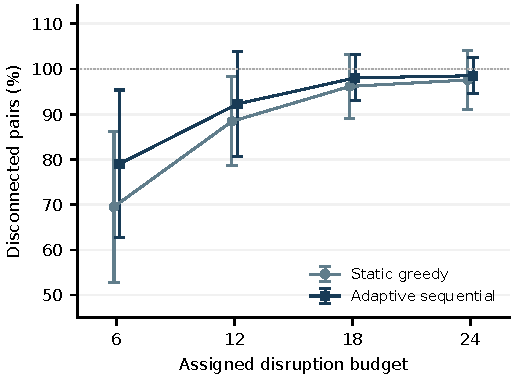
\includegraphics[width=\linewidth]{figures/revised_interdiction_results.pdf}
\caption{Measured disconnected-pair percentages on 30 generated graphs. Error bars show population SD across graphs. Horizontal values are assigned cost budgets. These are fixed-budget outcomes, not convergence trajectories.}
\label{fig:stackelberg_convergence}
\end{figure}

\paragraph{Operational Immutability Plateau and the Runtime Defense Residual}
In enterprise networks, a realistic fraction of directory edges represents immutable operational dependencies ($E_b \subsetneq E$). As shown in Table~\ref{tab:stackelberg_results} and Figure~\ref{fig:stackelberg_convergence}, proactive graph interdiction achieves \textbf{$98.5 \pm 4.0\%$} paths severed at $B_{\text{ops}}=24$ (vs. $97.6 \pm 6.5\%$ for Static Greedy).
This experiment leaves a mean residual of approximately $1.5\%$ under the selected graph instances, budgets, and non-blockable edges. It does not prove that every enterprise has an unavoidable residual of that size or that a different feasible policy cannot disconnect all modeled paths. Runtime monitoring is complementary to the evaluated hardening policies.

\paragraph{Paired tests and multiple comparisons}
Independent adjacency-list checks validate all 120 budget/cut outcomes and 11,100 reachability queries. Table~\ref{tab:stackelberg_results} compares adaptive and static greedy on the same 30 graphs using a paired $t$-test and exact signed-rank enumeration. The eight-test Holm family covers four budgets and two procedures~\cite{holm1979simple}. Budget 6 survives both procedures; budget 18 survives only exact signed rank (adjusted $p=0.02344$, paired-$t$ adjusted $p=0.05138$). At budget 24, only five paired differences are nonzero and all are positive. Exact enumeration over $2^5=32$ sign assignments gives raw $p=0.0625$; the mean gain is 0.94 percentage points. Both adjusted budget-24 values are $p=0.25$. The measurements therefore do not support a significant budget-24 difference. Ranks use exact rational disconnection fractions and omit zero differences. This is a descriptive synthetic-graph analysis, not evidence of enterprise operational superiority.

\paragraph{Revoked-edge count}
Under $B_{\text{ops}} = 24$, Static Greedy revokes an average of \textbf{10.9 edges} ($10.9 \pm 0.9$), under the assigned heterogeneous costs. The saved summary does not measure the resulting business-workflow disruption. The metadata-preserving adaptive rerun revokes an average of \textbf{5.7 edges} ($5.7 \pm 2.3$), a \textbf{47.7\% reduction in revoked-edge count}. The disruption weights are assigned model parameters; actual administrator effort and business disruption were not measured.

% Generated from the frozen repeated same-task projection experiment.
\begin{table}[ht]
\centering
\caption{Path-preserving projection with identical queried pairs: three graph seeds and five alternating-order timing repetitions per seed. Projection time is included. All reported severed-pair outcomes agree; these are hierarchical synthetic graphs on a shared host.}
\label{tab:scalability_bench}
\small
\begin{tabular}{rrrrr}
\toprule
Nodes & Queried pairs & Full (ms) & Projection + solve (ms) & Median ratio \\
\midrule
100 & 6 & 1.99 & 1.16 & $1.78\times$ \\
1,000 & 65 & 86.36 & 21.56 & $4.01\times$ \\
5,000 & 325 & 3448.15 & 439.29 & $7.54\times$ \\
\bottomrule
\end{tabular}
\end{table}


\paragraph{Scalability via Provenance-Cone Guidance}
We implement a path-preserving projection. For every requested pair $(s,t)$, retain the intersection of vertices reachable from $s$ and vertices that can reach $t$, together with every pair endpoint. Every original $s$--$t$ path is retained, so subsequent removal of any retained edge subset preserves that pair's reachability answer. Edge costs, relations and immutability are copied unchanged, and initially unconnected endpoints remain represented. Intersecting any full-graph cut with the retained edge set removes no requested-path effect and cannot increase its nonnegative cost, so the optimal budgeted pair-disconnection value is also preserved. A heuristic's selected cut can still depend on its search order. Shared endpoint closures are computed once per distinct endpoint.

The equal-query benchmark retains all pairs, uses the same sequential heuristic on full and projected graphs, and includes projection cost (Table~\ref{tab:scalability_bench}). At 5,000 actual nodes and 325 queried pairs, 874--890 nodes remain. Across fifteen alternating-order timing pairs, the median per-run ratio is $7.54\times$, with observed range $6.62$--$8.99\times$, and severed-pair outcomes agree in every run. The median full and projection-inclusive times are 3,448.15~ms and 439.29~ms; their ratio need not equal the median of individual ratios. This controlled result does not supply an optimality or enterprise workload guarantee.
